\documentclass[10pt,a4paper]{scrartcl}
\pagestyle{empty}
\usepackage{a4} % alternativ \usepackage{a4wide}
\usepackage[ngerman]{babel} % Neudeutsche Silbentrennung (mehrsprachiges Dokument)
\usepackage{parskip} % Skip indentation of first row
\usepackage{graphicx} % Graphics support
\usepackage{longtable} % Tables across several pages
\usepackage{booktabs}
\usepackage{hyperref} % Hyperlinks
\usepackage{float} % Force float position
\usepackage[automark]{scrpage2} %kopf/fusszeile
\usepackage[utf8x]{inputenc} % Unicode-Encoding
 
\linespread{1.3}

\author{Danilo Bargen, Christian Fässler, Jonas Furrer} 
\title{Qualitätsmanagement\\ Projekt BierIdee}

\pagestyle{scrheadings}
\ihead{SE2 Projekte} %linke Kopfzeile
\ohead{BierIdee} %rechte Kopfzeile

\begin{document}

\begin{titlepage}
	\maketitle
	\vspace{120mm}
	\thispagestyle{empty} % Don't start page numbers on this page
\end{titlepage}

\tableofcontents
\newpage

\section*{Änderungshistorie}
\begin{tabular}{p{0.1\textwidth}p{0.15\textwidth}p{0.55\textwidth}p{0.1\textwidth}}
\toprule
\textbf{Version} & \textbf{Datum} & \textbf{Änderung} & \textbf{Person} \\  
\midrule
v1.0 & 30.05.2012 & Dokument erstellt & dbargen \\  
\bottomrule
\end{tabular} 
\newpage


\section{Einführung}

\subsection{Zweck}
Dieses Dokument beschreibt die Qualitätssicherungsmassnahmen des Projektes BierIdee.

\subsection{Gültigkeitsbereich}
Die Gültigkeit des Dokumentes beschränkt sich auf die Dauer des SE2-Projekte Modules FS2012.

\subsection{Referenzen}

\begin{itemize}
	\item Definition.of.Done.pdf
	\item PullRequestExample.jpg
	\item usertest.baumann.pdf
	\item usertest.tanner.pdf
\end{itemize}


\newpage


\section{Definition of Done}

Als primäre Qualitätssicherungsmassnahme wurde eine Definition of Done\footnote{Siehe
\textit{Definition.of.Done.pdf}} erstellt. Diese enthält die im folgenden erwähnten
Qualitätsrelevanten Punkte.

\subsection{Code Reviews}

Um die Qualität der Codebasis zu gewährleisten, wurden regelmässig Code Reviews
durchgeführt. Gemäss Steve McConnell \cite{mcconnell2005code} ist dies eine äusserst effektive
Qualitätsmassnahme:

\begin{quote}
	[\ldots{}] software testing alone has limited effectiveness -- the average defect detection rate is only 25
	percent for unit testing, 35 percent for function testing, and 45 percent for integration testing.
	In contrast, the average effectiveness of design and code inspections are 55 and 60 percent. Case
	studies of review results have been impressive [\ldots]
\end{quote}

Gemäss der Definition of Done darf kein nichttrivialer Code in den \texttt{master} Branch gemerged
werden, ohne dass dieser reviewed wurde.

\subsubsection{Pull Requests}

Um die Code Reviews durchzuführen, wurde ein Feature von Github\footnote{\url{http://github.com/}}
eingesetzt, welches sich "`Pull Requests"` nennt. Der Workflow funktioniert folgendermassen:

\begin{enumerate}
	\item Ein Teammitglied will ein neues Feature entwickeln. Er erstellt mit Git einen neuen Branch
		und arbeitet darin.
	\item Wenn die Entwicklung des Features fertig ist oder er Feedback braucht, wird der Branch auf
		Github pushed.
	\item Auf Github erstellt das Teammitglied eine Anfrage, um den Branch in den \texttt{master}
		Branch zu megen (der sogenannte "`Pull Request"'). Der Pull Request ist ein Diskussionsthread,
		in welchem man den ganzen Branch, einzelne Commits oder einzelne Stellen im Code kommentieren
		kann.
	\item Wenn der Pull Request noch nicht merge-bereit ist, werden von einem Teammitglied im Branch
		weitere Commits erstellt. Sobald sie auf Github pushed werden, erscheinen sie auch im Pull
		Request.
	\item Wenn alle mit dem Code zufrieden sind, wird er mit dem \texttt{master} Branch gemerged.
		Falls der Merge konfliktfrei möglich ist, kann dies direkt über das Webinterface von Github
		gemacht werden.
\end{enumerate}

Mit diesem Workflow konnten wir Frontend, Backend wie auch die LaTeX-Dokumente reviewen,
überarbeiten und laufend verbessern. Ein grosser Vorteil daran ist vor allem, dass man direkt im
Code-Diff Diskussionen erstellen kann.

\begin{figure}[H]
	\begin{center}
		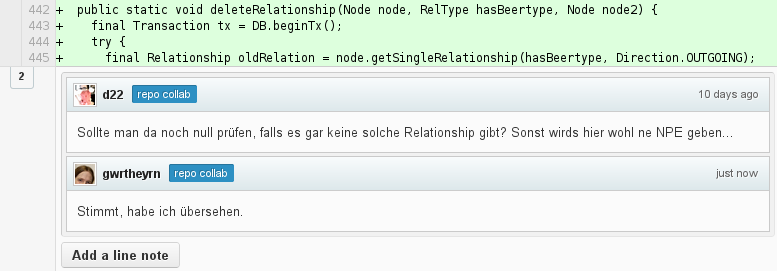
\includegraphics[width=\textwidth]{img/github2.png}
	\end{center}
	\caption{Diskussion im Diff}
\end{figure}

Die Github-Gruppe für unser Projekt kann online\footnote{\url{https://github.com/bieridee}}
eingesehen werden.

\begin{figure}[H]
	\begin{center}
		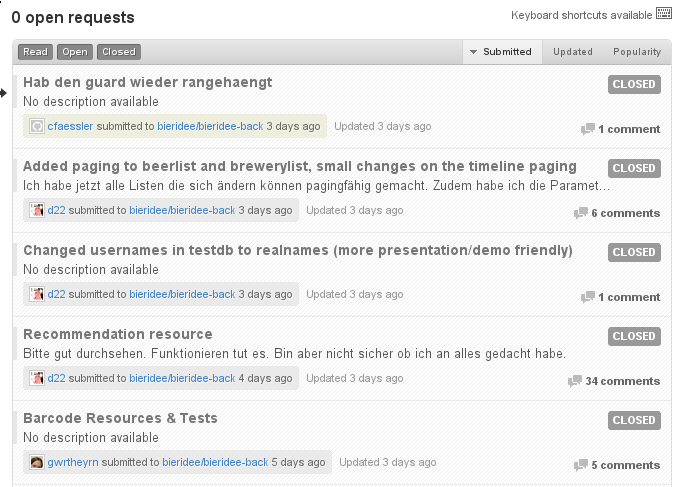
\includegraphics[width=\textwidth]{img/github1.png}
	\end{center}
	\caption{Backend Pull Requests (Auszug)}
\end{figure}

Ein erweitertes Beispiel einer Pull Request Diskussion findet sich in der Datei
\texttt{PullRequestExample.jpg}.

\subsection{Code-Kommentare}

Um die Codebasis übersichtlich und gut verständlich zu halten, sollten überall wo sinnvoll
Code-Kommentare eingefügt werden. Klassen und Methoden müssen mit Javadoc kommentiert werden. Daraus
wird nach Abschluss des Projektes eine Javadoc-HTML-Hilfe generiert.

\subsection{Checkstyle}

Während des Projektes wurde Checkstyle\footnote{\url{http://checkstyle.sourceforge.net/}} mit
einer eigens für das Projekt erstellen Konfigureation eingesetzt. Um die Definition of Done zu
erfüllen, dürfen im Code mithilfe dieser Checkstyle-Konfiguration keine Warnungen mehr vorhanden
sein. 

\subsection{Unit Tests}

Unit Tests müssen vorhanden sein, um die neu erstellte Funktionalität zu testen. Im Backend wurde
dafür JUnit 4 eingesetzt, im Frontend JUnit 3 mit
Robotium\footnote{\url{http://code.google.com/p/robotium/}}.

\subsection{Continuous Integration}

Damit die Codebasis stets kompilierbar bleibt, wurde ein Jenkins Buildserver eingesetzt. Dieser
wurde mit diversen Plugins erweitert (Github Plugin, Maven Plugin, Android Plugin, etc\ldots). Neben
dem Buildvorgang wurden auch die Unit- und Integrationtests ausgeführt. Um die
Android-Integrationstests auszuführen wurde im Hintergrund jeweils eine VNC-Server-Instanz
gestartet, die den Emulator gestartet und die Tests darin ausgeführt hat.

Zu Beginn des Projektes wurde zudem vereinbart, dass ein durch Unachtsamkeit verschuldeter Build Fail
bestraft wird -- die entsprechende Person muss am nächsten Tag Gipfeli für das Team mitbringen.

\begin{figure}[H]
	\begin{center}
		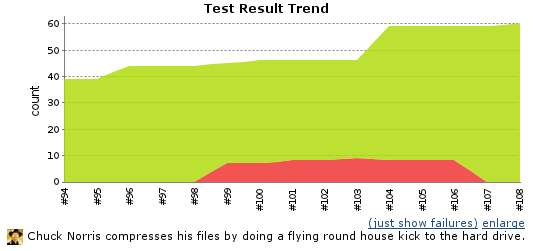
\includegraphics[width=0.8\textwidth]{img/jenkins1.png}
	\end{center}
	\caption{Test Result-Trend Backend}
\end{figure}

\begin{figure}[H]
	\begin{center}
		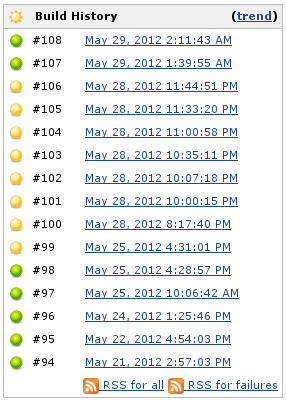
\includegraphics[height=0.7\textwidth]{img/jenkins2.png}
	\end{center}
	\caption{Build-History Backend}
\end{figure}

Die Continuous Integration verlief leider nicht so reibungslos wie erwartet. Durch Probleme mit dem
Caching der Codebasis (das Repository wurde nicht jedesmal neu ausgecheckt sondern nur updated) war
der Build-Status auf dem Integrationsserver (vor Allem im Frontend-Projekt) häufig auf "`Fehlerhaft"',
obwohl der Build wie auch alle Tests eigentlich erfolgreich durchführbar waren. Diese Probleme
wurden jeweils durch ein manuelles "`cleaning"' des Workspace gelöst.

\section{Issue Tracking}

Um den Überblick über die geplanten Tasks zu behalten und um sicherzustellen, dass keine Features
vergessen gehen, wurde während dem Projekt konsequent mit Redmine gearbeitet. Alle Aufgaben wurden
in Tasks unterteilt und den jeweiligen Personen zugeteilt. Zeitschätzungen wurden eingetragen und
Kategorien gesetzt.

\begin{figure}[H]
	\begin{center}
		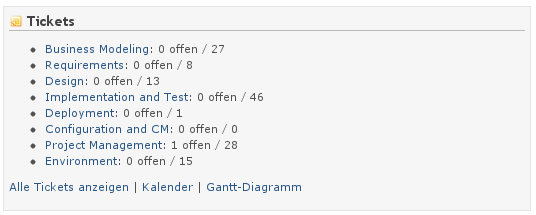
\includegraphics[width=0.8\textwidth]{img/redmine.png}
	\end{center}
	\caption{Redmine Ticket-Statistik}
\end{figure}

\section{Usertests}

Um auch Feedback von Benutzern zu erhalten und so auf Probleme aufmerksam zu werden die man als
Entwickler häufig übersieht, haben wir ein Testprotokoll erstellt und die App von Freiwilligen
testen lassen. Die Erkenntnisse flossen jeweils direkt in den Entwicklungszyklus ein.

Zwei Beispiele sind in in den PDF-Dateien \texttt{usertest.\-baumann.\-pdf} und
\texttt{usertest.\-tanner.\-pdf} beigefügt.

\section{Protokolle}

Für jedes Meeting wurde jeweils ein Protokoll erstellt. Zu Beginn haben wir dafür die Website
http://minutes.io/ verwendet, später wurde wegen Bugs auf deren Website auf Textdateien
umgestellt.


\bibliographystyle{alpha}
\bibliography{QA}


\end{document}
